\noindent

\includegraphics[height=1.25cm]{images/pictograms/benchmark}

\includegraphics[height=1.25cm]{images/pictograms/FEM}

\includegraphics[height=1.25cm]{images/pictograms/paraview}

%%%%%%%%%%%%%%%%%%%%%%%%%%%%%%%%%%%%%%%%%%%%%%%%%%%%%%%%%%%%%%%%%%%%%%%%%%%%%%%%%%%%%%%%%%%%%%%%%%%

\begin{flushright} {\tiny {\color{gray} python\_codes/fieldstone\_76/text.tex}} \end{flushright}


\par\noindent\rule{\textwidth}{0.4pt}

\begin{center}
\inpython
{\small Code: \url{https://github.com/cedrict/fieldstone/tree/master/python_codes/fieldstone_76}}
\end{center}

%\par\noindent\rule{\textwidth}{0.4pt}
%{\sl This stone was developed in collaboration with Donald Duck}. \index{contributors}{D. Duck}

\par\noindent\rule{\textwidth}{0.4pt}

Last revision: Feb. 15th, 2025.

\par\noindent\rule{\textwidth}{0.4pt}

%%%%%%%%%%%%%%%%%%%%%%%%%%%%%%%%%%%%%%%%%%%%%%%%%%%%%%%%%%%%%%%%%%%%%%%%%%%%%%%%%%%%%%%%%%%%%%%%%%%


This stone is an example of $Q_2\times P_{-1}$ implementation. 
The 2d $Q_2$ shape functions have been derived in Section~\ref{MMM-ss:q22d}
The $-1$ subscript indicates that the pressure field is linear (but not bilinear!)
as explained in Section~\ref{MMM-sec:terminology}.

%............................................................
\subsection*{Mapped vs un-mapped pressure basis functions}

Actually the story is a bit more complicated than that, as explained for 
example in \textcite{boga02} (2002):
\begin{displayquote}
{\color{darkgray}
Two possible choices are given for the definition of the pressure space: 
one can either use a global pressure approximation (that is on
each quadrilateral the finite element space is spanned by 1 and by the 
global co-ordinates $x$ and $y$) or a local approach (consisting in generating 
the local space by means of the constants and the local curvilinear 
co-ordinates on each quadrilateral $r$ and $s$). [...] Numerical results 
actually show that the second choice (local or mapped pressure approximation) 
is suboptimally convergent.
}
\end{displayquote}

In other words, the mapped version consists of  
using the $P_{-1}$ basis functions defined in Section~\ref{MMM-ss:lbfq2D}:
inside the reference element the pressure is given by $p^h(r,s)=a+br+cs$ 

The unmapped version is a bit less straightforward and is as follows:
let us assume there are three pressure nodes inside the element.
Inside each element the pressure is defined by a linear field
\[
p^h(x,y) = a+bx+cy
\]
We must then compute the coefficients $a,b,c$. We know that 
the expression above evaluated at the pressure nodes with 
coordinates $(x_i,y_i)$ should be equal to $p_i$. 
Then we have the following three equations:
\begin{eqnarray}
a + bx_1 + cy_1 &=& p_1 \nn\\
a + bx_2 + cy_2 &=& p_2 \nn\\
a + bx_3 + cy_3 &=& p_3 \nn
\end{eqnarray}
or, 
\[
\left(
\begin{array}{ccc}
1 & x_1 & y_1 \\
1 & x_2 & y_2 \\
1 & x_3 & y_3 
\end{array}
\right)
\cdot 
\left(
\begin{array}{ccc}
a \\ b \\ c
\end{array}
\right)
=
\left(
\begin{array}{ccc}
p_1 \\ p_2 \\ p_3
\end{array}
\right)
\]
Then 
\[
\left(
\begin{array}{ccc}
a \\ b \\ c
\end{array}
\right)
=
\left(
\begin{array}{ccc}
1 & x_1 & y_1 \\
1 & x_2 & y_2 \\
1 & x_3 & y_3 
\end{array}
\right)^{-1}
\cdot
\left(
\begin{array}{ccc}
p_1 \\ p_2 \\ p_3
\end{array}
\right)
= {\bm M}^{-1} \cdot \vec{p}
\]
with 
\[
{\bm M}^{-1} = \frac{1}{\Delta}
\left(
\begin{array}{ccc}
x_2y_3-x_3y_2 & x_3y_1-x_1y_3 & x_1y_2-x_2y_1 \\
y_2-y_3 & y_3-y_1 & y_1-y_2 \\
x_3-x_2 & x_1-x_3 & x_2-x_1
\end{array}
\right)
=
\left(
\begin{array}{ccc}
m_{11} & m_{12} & m_{13} \\
m_{21} & m_{22} & m_{23} \\
m_{31} & m_{32} & m_{33} 
\end{array}
\right)
\]
and
\[
\Delta = x_2y_3-x_3y_2 - x_1y_3-x_3y_1 + x_1y_2-x_2y_1
\]
so that
\begin{eqnarray}
a &=& m_{11}p_1 + m_{12} p_2 + m_{13} p_3 \nn\\
b &=& m_{21}p_1 + m_{22} p_2 + m_{23} p_3 \nn\\
c &=& m_{31}p_1 + m_{32} p_2 + m_{33} p_3 \nn
\end{eqnarray}
In the end 
\begin{eqnarray}
p^h(x,y) 
&=&  a+bx+cy \nn\\
&=& m_{11}p_1 + m_{12} p_2 + m_{13} p_3
+ (m_{21}p_1 + m_{22} p_2 + m_{23} p_3) x
+ (m_{31}p_1 + m_{32} p_2 + m_{33} p_3) y \nn\\
&=& \underbrace{(m_{11} + m_{21}x + m_{31}y)}_{\bN_1(x,y)} p_1 
+   \underbrace{(m_{12} + m_{22}x + m_{32}y)}_{\bN_2(x,y)} p_2 
+   \underbrace{(m_{13} + m_{23}x + m_{33}y)}_{\bN_3(x,y)} p_3
\end{eqnarray}
The basis functions are then evaluated at the (real) coordinates 
of the quadrature point $(x_q,y_q)$.



%..............................................................................
\subsection*{About the code}

For all the tests/benchmarks the box is a unit square.
Velocity nodes coordinates are stored in the \lstinline{xV,yV} arrays
with the \lstinline{iconV} connectivity array.
Pressure nodes coordinates are stored in the \lstinline{xP,yP} arrays
with the \lstinline{iconP} connectivity array.

The mesh counts \lstinline{nel=nelx*nely} elements,
\lstinline{NV=(2*nelx+1)*(2*nely+1)} velocity nodes and 
\lstinline{NP=3*nel} pressure nodes.

The \lstinline{meth} parameter is 1 for mapped approach and 2 
for un-mapped approach. 

The parameter \lstinline{xi} controls the randomness of the mesh as follows:
for each node inside the domain (i.e. not on the boundaries) a random value 
in the range $[-\xi,\xi]$ is added to the $x$ and $y$ coordonates:
\begin{lstlisting}
for i in range(0,NV):
    if xV[i]>0 and xV[i]<Lx and yV[i]>0 and yV[i]<Ly:
       xV[i]+=random.uniform(-1.,+1)*hx*xi
       yV[i]+=random.uniform(-1.,+1)*hy*xi
\end{lstlisting}
If $\xi=0$ then no randomness is added to the nodes position and the 
mesh consists of rectangular elements (and for simplicity of square elements).

Another mesh deformation approach is borrowed from \stone~25 which models the 
Rayleigh-Taylor experiment of \textcite{vaks97} (1997). Only the vertical position 
of the nodes is modified.


When mesh randomization or mesh deformation is added to all nodes, 
I make sure that the velocity nodes 4,5,6,7 in the middle of the edges 
are really put back between nodes 0-1, 1-2, 2-3, and 3-0 respectively. 
The node in the middle of the element is also then moved accordingly.
\begin{lstlisting}
for iel in range(0,nel):
    xV[iconV[4,iel]]=0.5*(xV[iconV[0,iel]]+xV[iconV[1,iel]])
    yV[iconV[4,iel]]=0.5*(yV[iconV[0,iel]]+yV[iconV[1,iel]])
    xV[iconV[5,iel]]=0.5*(xV[iconV[1,iel]]+xV[iconV[2,iel]])
    yV[iconV[5,iel]]=0.5*(yV[iconV[1,iel]]+yV[iconV[2,iel]])
    xV[iconV[6,iel]]=0.5*(xV[iconV[2,iel]]+xV[iconV[3,iel]])
    yV[iconV[6,iel]]=0.5*(yV[iconV[2,iel]]+yV[iconV[3,iel]])
    xV[iconV[7,iel]]=0.5*(xV[iconV[3,iel]]+xV[iconV[0,iel]])
    yV[iconV[7,iel]]=0.5*(yV[iconV[3,iel]]+yV[iconV[0,iel]])
    xV[iconV[8,iel]]=0.25*(xV[iconV[0,iel]]+xV[iconV[1,iel]]+xV[iconV[2,iel]]+xV[iconV[3,iel]])
    yV[iconV[8,iel]]=0.25*(yV[iconV[0,iel]]+yV[iconV[1,iel]]+yV[iconV[2,iel]]+yV[iconV[3,iel]])
\end{lstlisting}

The three types of meshes are shown here:

\begin{center}
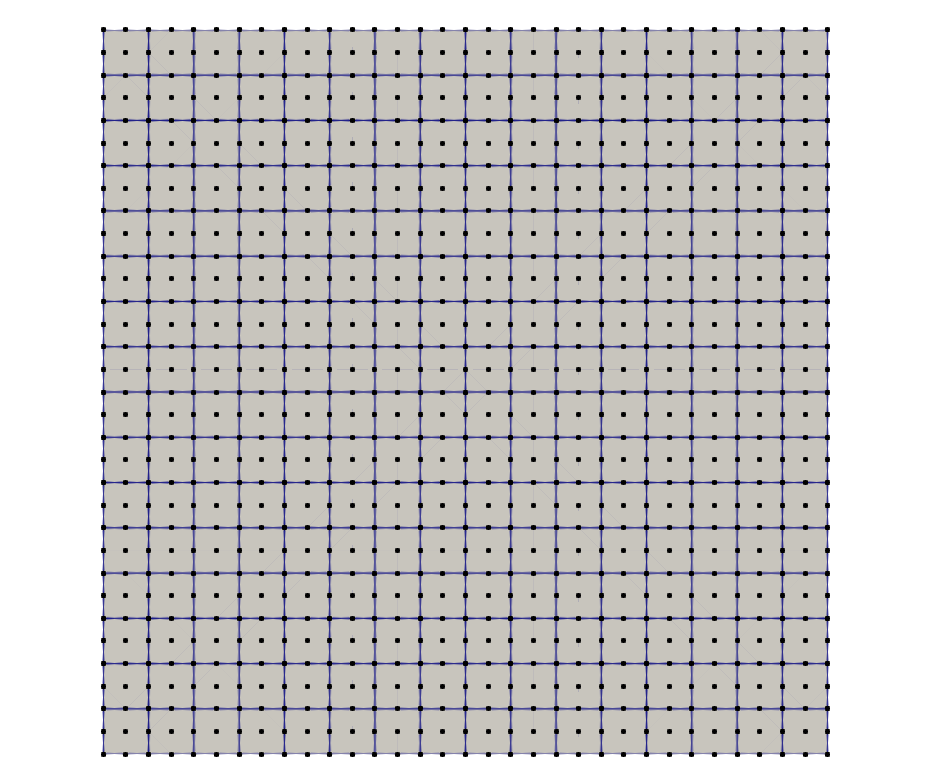
\includegraphics[width=5.7cm]{python_codes/fieldstone_76/results/mesh_type1}
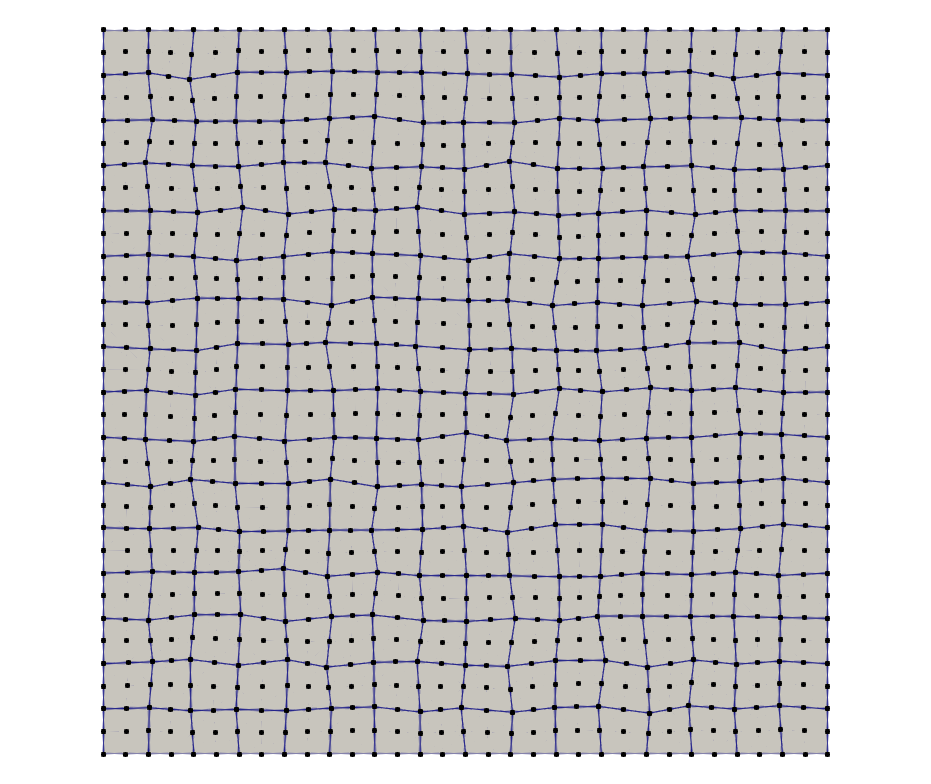
\includegraphics[width=5.7cm]{python_codes/fieldstone_76/results/mesh_type2}
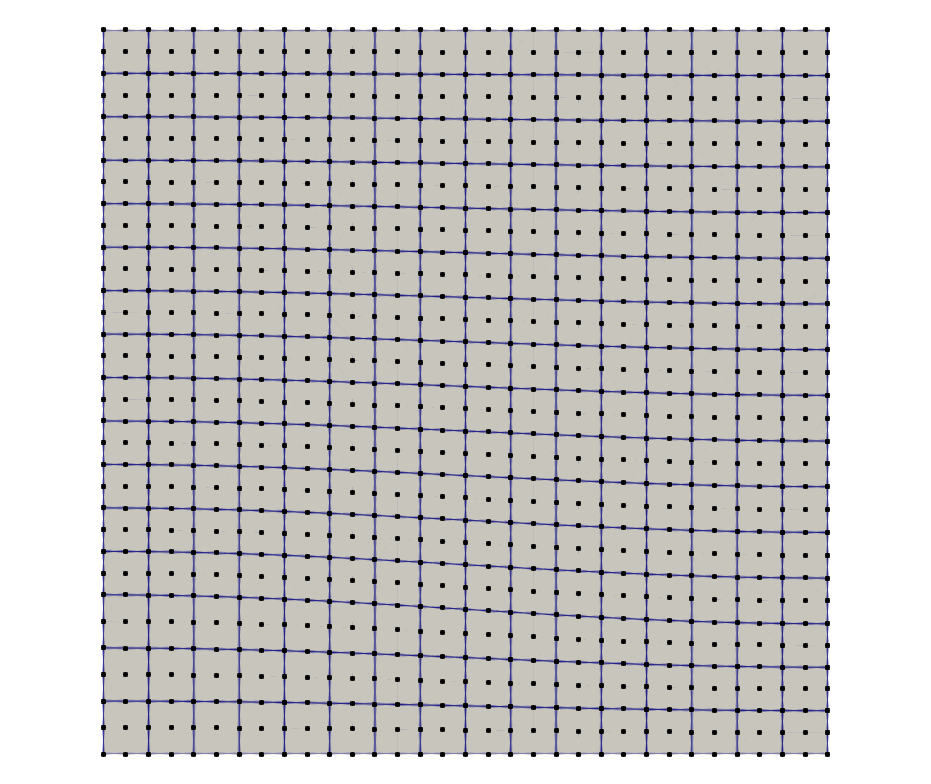
\includegraphics[width=5.7cm]{python_codes/fieldstone_76/results/mesh_type3}\\
{\captionfont From left to right: mesh types 1, 2, and 3, or 'square', 'random' 
and 'wave' meshes.}
\end{center}

The mapping is isoparametric (i.e. $Q_2$). The same mapping is used for all integrals.
In the case of rectangular elements both the mapped and un-mapped approaches 
yield the same pressure basis functions values at the quadrature points
so the measured errors and vrms are identical.
{\color{red} what about trapezes? parallelograms?} 

The same quadrature rule is used for $\K$ and $\G$ blocks.
I explore the effect of the number of quadrature points on the solution, 
so I allow for $2^2$, $3^2$ and $4^2$ quadrature points
as parameterized by the \lstinline{nqperdim} parameter. 

One source of uncertainty on my part is how/where to setup the pressure nodes.
For mapped elements the $P_{-1}$ pressure basis functions are defined as 
\begin{lstlisting}
def NNP(r,s):
    NP_0=1-r-s
    NP_1=r
    NP_2=s
    return np.array([NP_0,NP_1,NP_2],dtype=np.float64)
\end{lstlisting}
In other words the first pressure node is at coordinates $(0,0)$,
the second at $(1,0)$ and the third at $(0,1)$ inside the reference element $[-1,+1]^2$.

For the un-mapped version we need to define the pressure node coordinates 
directly in the $x,y$-axis system.
At the moment it is done as follows: The ninth velocity node of the element is 
in the center of the element and is also the first pressure node.
Since the elements are marginally deformed I can place the second pressure node 
a distance $h_x/2$ in the $x$-direction from the first point, and the third pressure node 
a distance $h_y/2$ in the $y$-direction from the first point.

\begin{lstlisting}
counter=0
for iel in range(nel):
    xP[counter]=xV[iconV[8,iel]]
    yP[counter]=yV[iconV[8,iel]]
    counter+=1
    xP[counter]=xV[iconV[8,iel]]+hx/2
    yP[counter]=yV[iconV[8,iel]]
    counter+=1
    xP[counter]=xV[iconV[8,iel]]
    yP[counter]=yV[iconV[8,iel]]+hy/2
    counter+=1
\end{lstlisting}
In this case the pressure basis functions need to be computed
element by element:

\begin{lstlisting}
for iel in range(0,nel):
    if meth==2:
       det=xP[iconP[1,iel]]*yP[iconP[2,iel]]-xP[iconP[2,iel]]*yP[iconP[1,iel]]\
          -xP[iconP[0,iel]]*yP[iconP[2,iel]]+xP[iconP[2,iel]]*yP[iconP[0,iel]]\
          +xP[iconP[0,iel]]*yP[iconP[1,iel]]-xP[iconP[1,iel]]*yP[iconP[0,iel]]
       m11=(xP[iconP[1,iel]]*yP[iconP[2,iel]]-xP[iconP[2,iel]]*yP[iconP[1,iel]])/det
       m12=(xP[iconP[2,iel]]*yP[iconP[0,iel]]-xP[iconP[0,iel]]*yP[iconP[2,iel]])/det
       m13=(xP[iconP[0,iel]]*yP[iconP[1,iel]]-xP[iconP[1,iel]]*yP[iconP[0,iel]])/det
       m21=(yP[iconP[1,iel]]-yP[iconP[2,iel]])/det
       m22=(yP[iconP[2,iel]]-yP[iconP[0,iel]])/det
       m23=(yP[iconP[0,iel]]-yP[iconP[1,iel]])/det
       m31=(xP[iconP[2,iel]]-xP[iconP[1,iel]])/det
       m32=(xP[iconP[0,iel]]-xP[iconP[2,iel]])/det
       m33=(xP[iconP[1,iel]]-xP[iconP[0,iel]])/det
\end{lstlisting}


In the near future I want to try elements that 
showcase curves edges. How am I to place P nodes ??

In both cases (mapped and un-mapped) the pressure is discontinuous from an element to another 
and this poses a little problem in terms of exporting it to 
vtu (and plotting with paraview). 
I then simply choose to export the value of the pressure in the middle of 
each element. {\color{red} I should improve this in the future, but it is 
only a visualisation problem.}


Quick summary of what follows without going into 
much detail: I carry out three benchmarks based on manufactured solutions  
and recover the expected cubic convergence for the velocity error 
and a quadratic error convergence for the pressure 
\textit{only} for the unmapped approach
in the case of non-rectangular elements.


profiles dont work with unmapped


\newpage
%.......................................................
\subsection*{Manufactured solution of Donea \& Huerta ({\tt bench=3})}

This is the Donea \& Huerta benchmark that is fully described in Section~\ref{MMM-mms1}.

\begin{eqnarray}
u(x,y) &=& x^2(1-x)^2 2y (y-1)(2y-1) \nonumber\\
v(x,y) &=& -y^2 (1 - y)^2 2x (x-1)(2x-1) \nonumber\\
p(x,y) &=& x(1 -x)- 1/6 \nonumber 
\end{eqnarray}
Note that the pressure obeys $\int_{\Omega} p \; dV = 0$.


\begin{center}
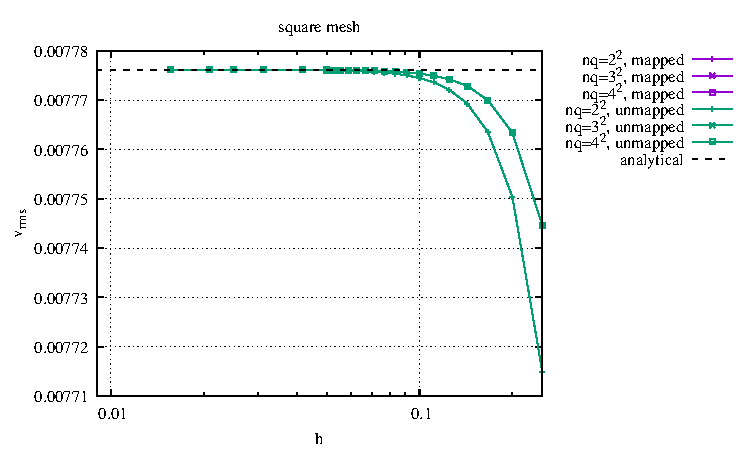
\includegraphics[width=5.7cm]{python_codes/fieldstone_76/results/bench3/reg/vrms}
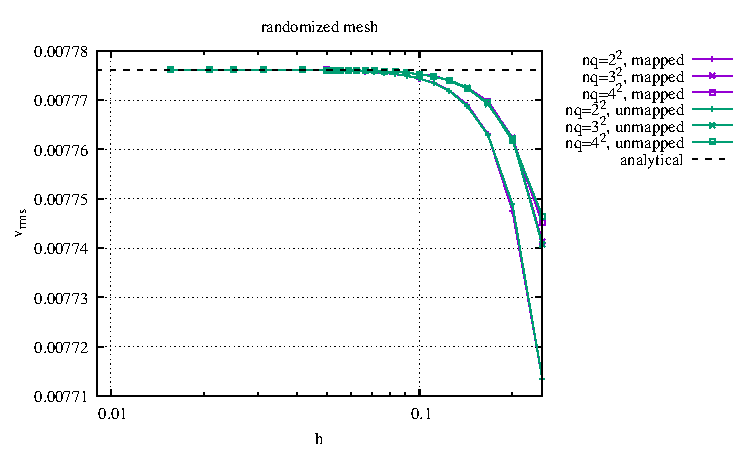
\includegraphics[width=5.7cm]{python_codes/fieldstone_76/results/bench3/rand/vrms}
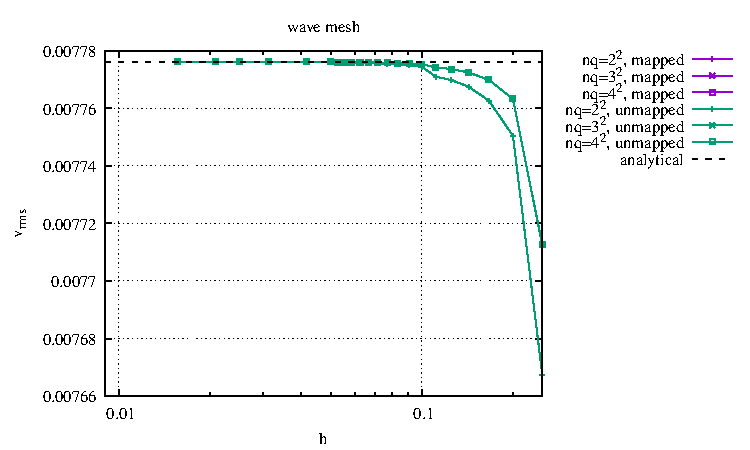
\includegraphics[width=5.7cm]{python_codes/fieldstone_76/results/bench3/wave/vrms}\\
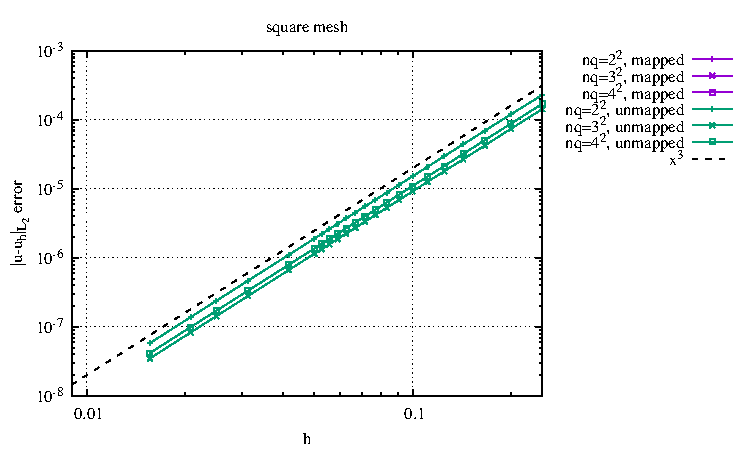
\includegraphics[width=5.7cm]{python_codes/fieldstone_76/results/bench3/reg/errors_V}
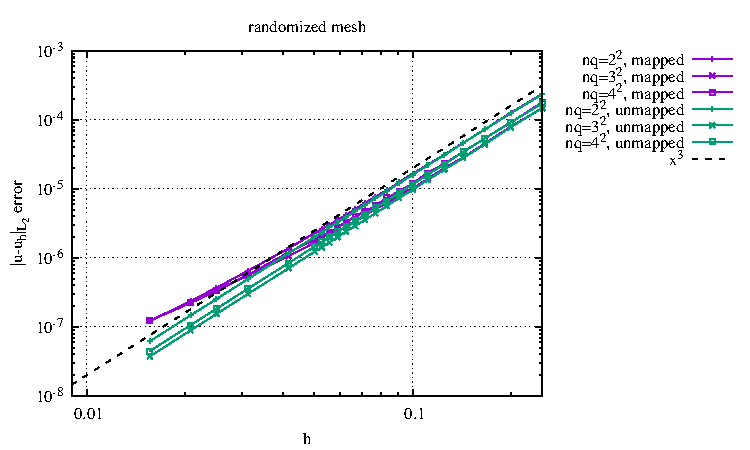
\includegraphics[width=5.7cm]{python_codes/fieldstone_76/results/bench3/rand/errors_V}
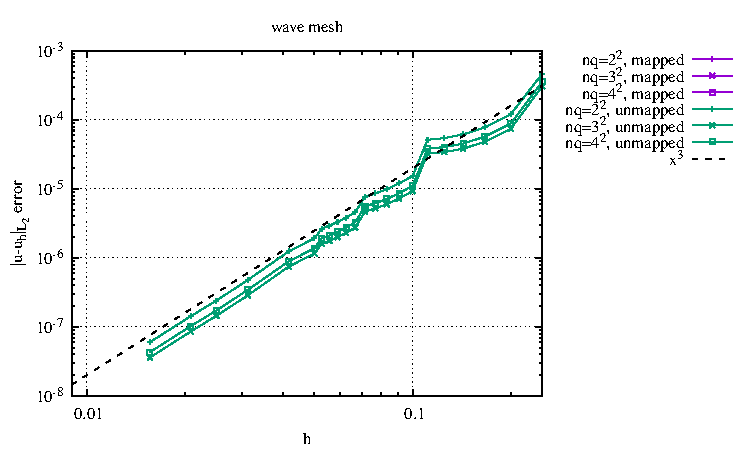
\includegraphics[width=5.7cm]{python_codes/fieldstone_76/results/bench3/wave/errors_V}\\
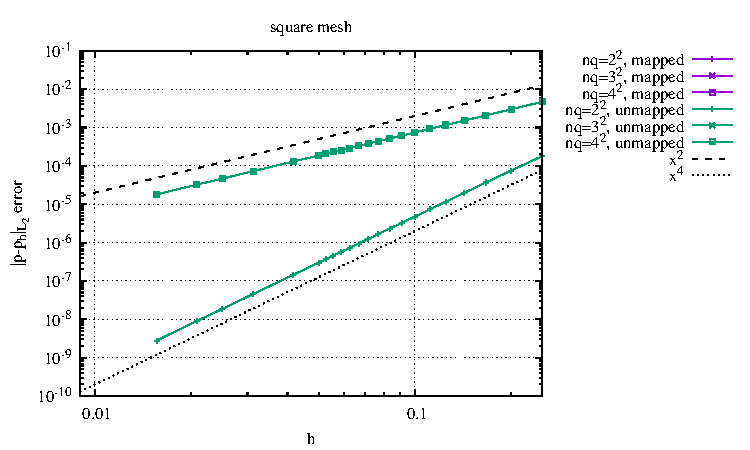
\includegraphics[width=5.7cm]{python_codes/fieldstone_76/results/bench3/reg/errors_P}
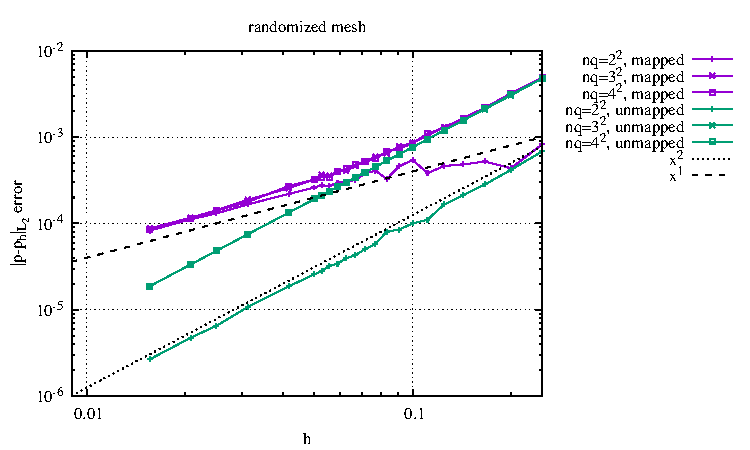
\includegraphics[width=5.7cm]{python_codes/fieldstone_76/results/bench3/rand/errors_P}
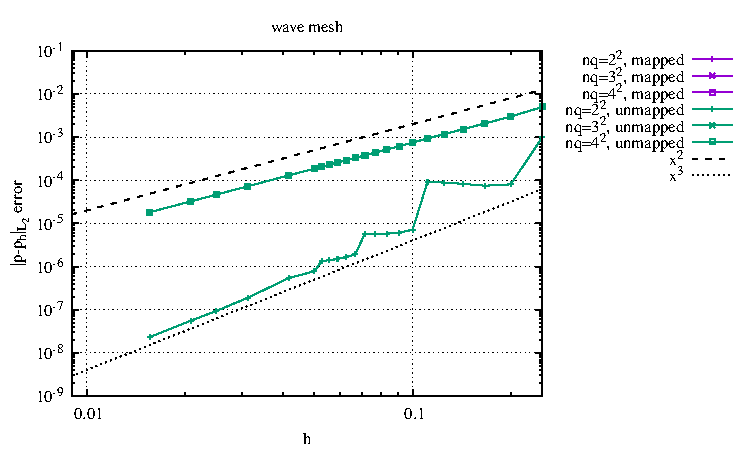
\includegraphics[width=5.7cm]{python_codes/fieldstone_76/results/bench3/wave/errors_P}\\
{\captionfont Left column: Regular square mesh; middle column: Randomized $\xi=0.1$ mesh;
right column: wave mesh.}
\end{center}

Remark: This is rather peculiar. I seem to recover 
a 4th order convergence for the pressure error when 
$2\times 2$ quadratures are used but not higher order ones...? 
This does not happen with either randomised meshes or 
other manufactured solutions so I will attribute this superconvergence 
to the fact that the pressure field is independent 
of $y$ and is only a second order polynomial in $x$ and elements are all square. 

\newpage
%......................................................
\subsection*{Manufactured solution \#1 ({\tt bench=1})}

The analytical solution originates in Lamichhane (2017) \cite{lami17}.
The velocity and pressure are given by
\begin{eqnarray}
u(x,y)&=&-2x^2y(2y-1)(x-1)^2(y-1) \\
v(x,y)&=& 2xy^2(2x-1)(x-1)(y-1)^2 \\
p(x,y)&=& x(1-x)(1-2y)
\end{eqnarray}
Boundary conditions are no-slip on all sides of the unit square. 
The corresponding body force terms are derived in Section~\ref{MMM-ss:mms11}. 

\begin{center}
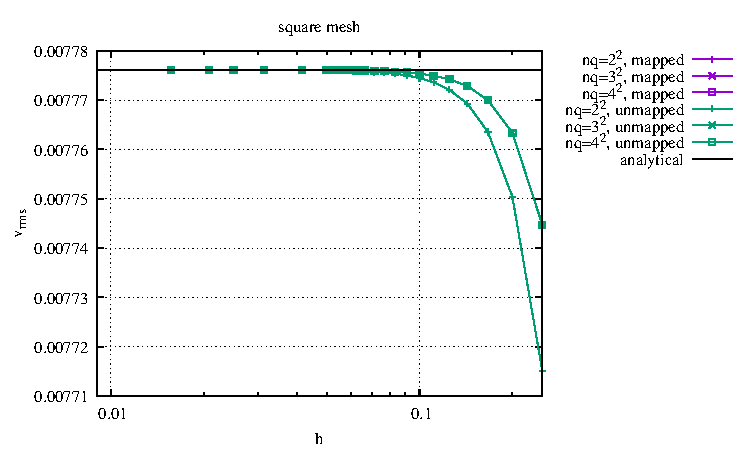
\includegraphics[width=5.7cm]{python_codes/fieldstone_76/results/bench1/reg/vrms}
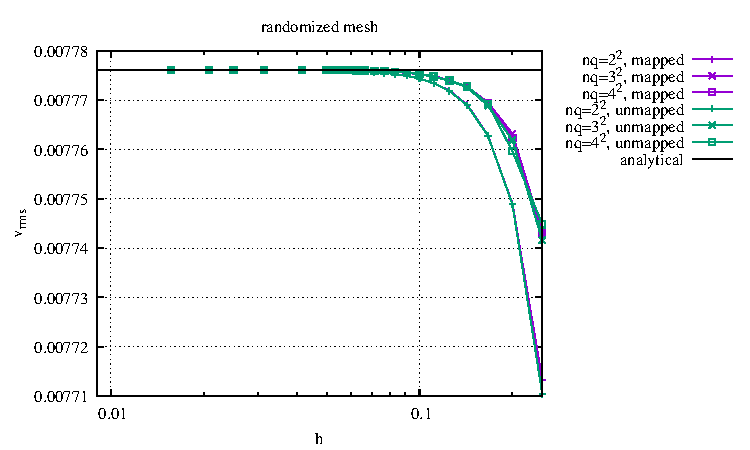
\includegraphics[width=5.7cm]{python_codes/fieldstone_76/results/bench1/rand/vrms}
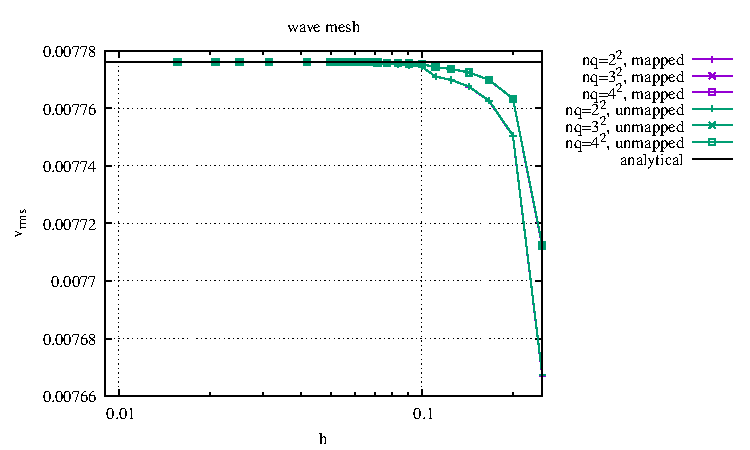
\includegraphics[width=5.7cm]{python_codes/fieldstone_76/results/bench1/wave/vrms}\\
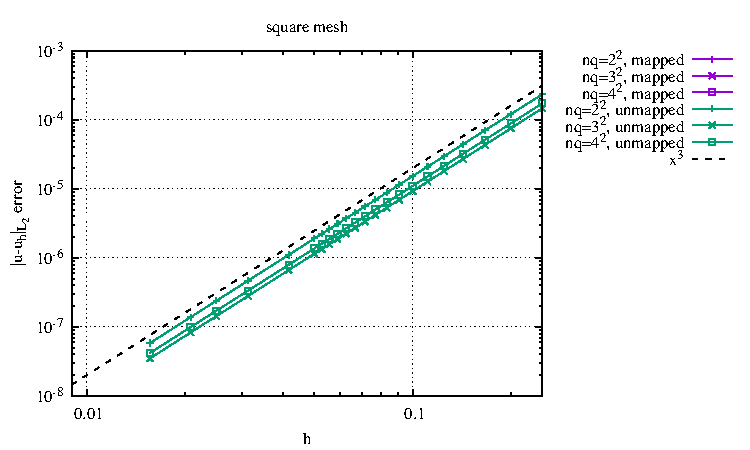
\includegraphics[width=5.7cm]{python_codes/fieldstone_76/results/bench1/reg/errors_V}
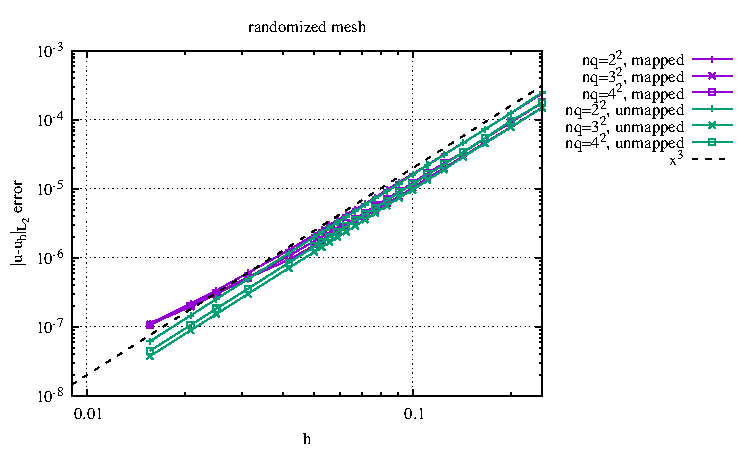
\includegraphics[width=5.7cm]{python_codes/fieldstone_76/results/bench1/rand/errors_V}
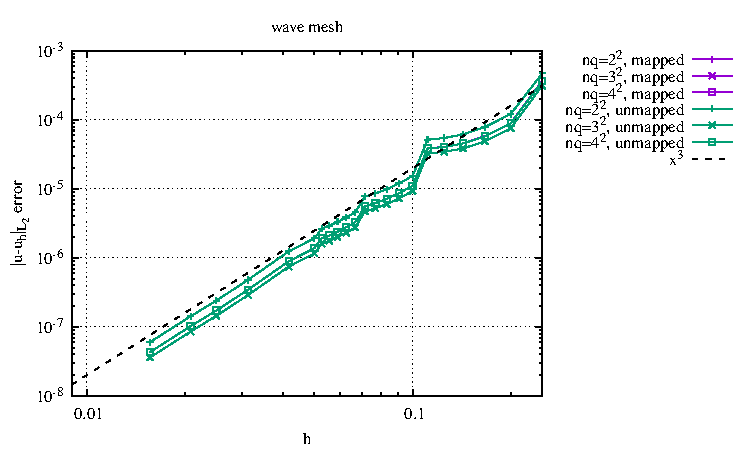
\includegraphics[width=5.7cm]{python_codes/fieldstone_76/results/bench1/wave/errors_V}\\
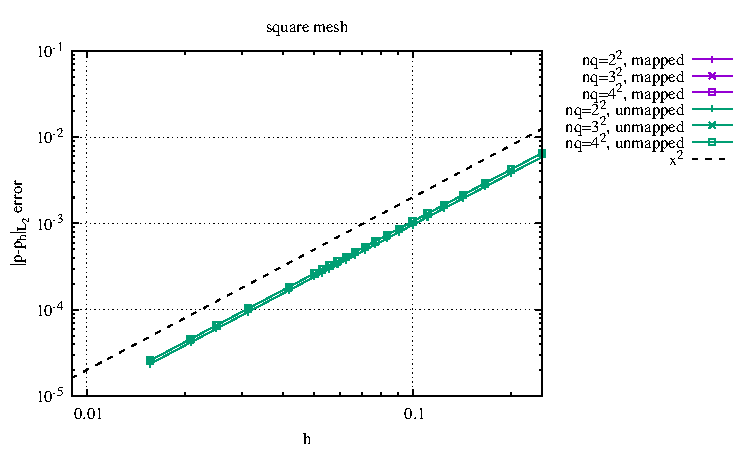
\includegraphics[width=5.7cm]{python_codes/fieldstone_76/results/bench1/reg/errors_P}
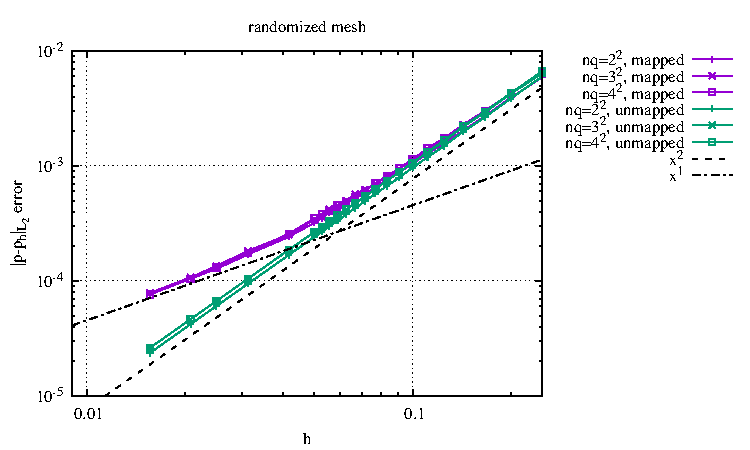
\includegraphics[width=5.7cm]{python_codes/fieldstone_76/results/bench1/rand/errors_P}
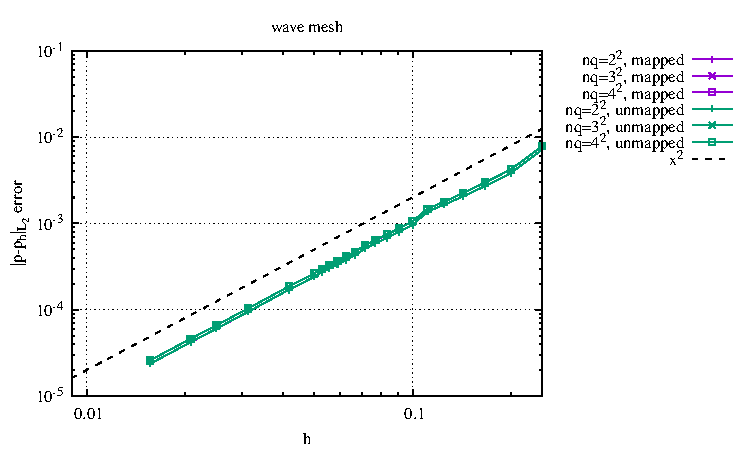
\includegraphics[width=5.7cm]{python_codes/fieldstone_76/results/bench1/wave/errors_P}\\
{\captionfont Left column: Regular square mesh; middle column: Randomized $\xi=0.1$ mesh;
right column: wave mesh.}
\end{center}

\newpage
%......................................................
\subsection*{Manufactured solution \#2 ({\tt bench=9})}

This is the second manufactured solution 
mentioned in Lamichhane \cite{lami17}. It is presented in Section~\ref{MMM-ss:mms2}.
It is for a unit square with $\eta=1$ and the smooth exact solution is
\begin{eqnarray}
u(x,y) &=& x+x^2 - 2xy+x^3 - 3xy^2 + x^2y \\
v(x,y) &=& -y-2xy+y^2 -3x^2y + y^3 - xy^2 \\
p(x,y) &=& xy+x+y+x^3y^2 - 4/3
\end{eqnarray}
Note that the pressure obeys $\int_{\Omega} p \; dV = 0$. The analytical 
velocity is prescribed on the boundary of the domain. 

\begin{center}
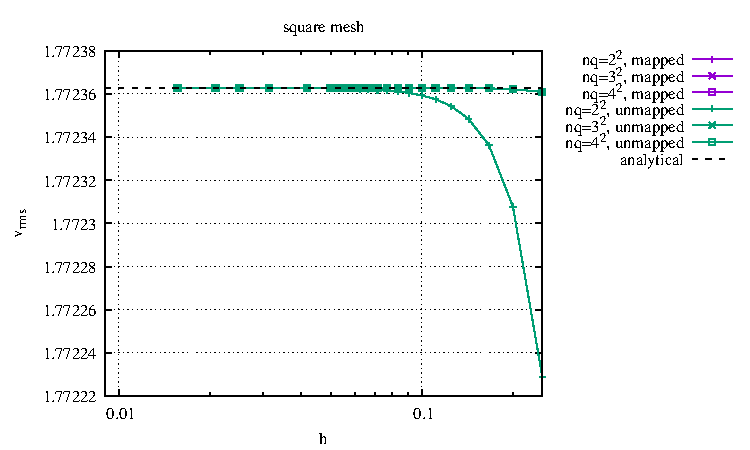
\includegraphics[width=5.7cm]{python_codes/fieldstone_76/results/bench9/reg/vrms}
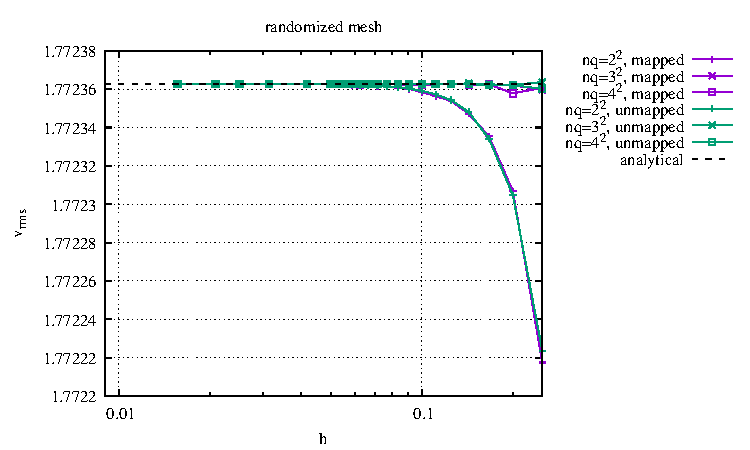
\includegraphics[width=5.7cm]{python_codes/fieldstone_76/results/bench9/rand/vrms}
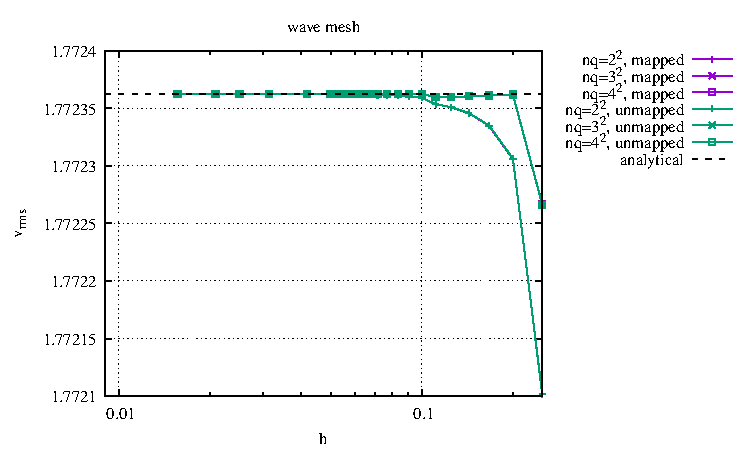
\includegraphics[width=5.7cm]{python_codes/fieldstone_76/results/bench9/wave/vrms}\\
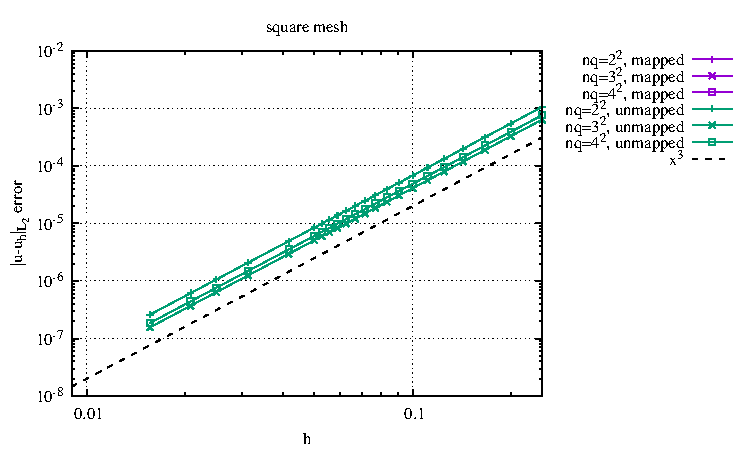
\includegraphics[width=5.7cm]{python_codes/fieldstone_76/results/bench9/reg/errors_V}
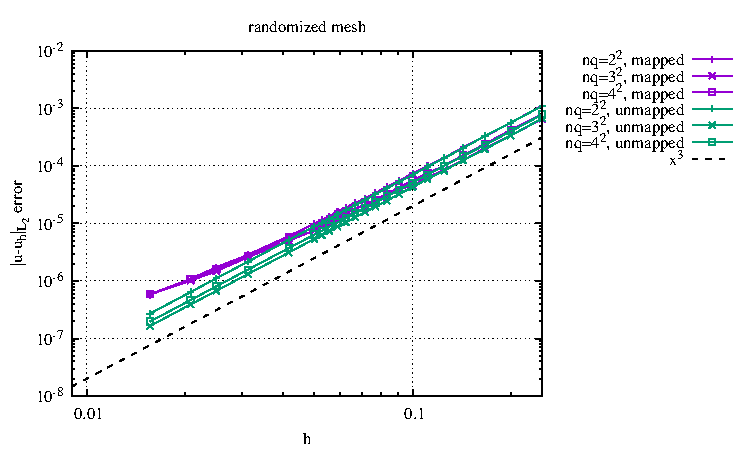
\includegraphics[width=5.7cm]{python_codes/fieldstone_76/results/bench9/rand/errors_V}
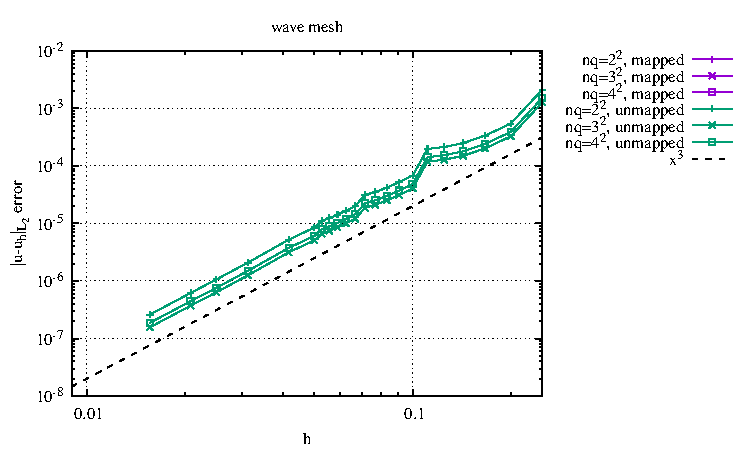
\includegraphics[width=5.7cm]{python_codes/fieldstone_76/results/bench9/wave/errors_V}\\
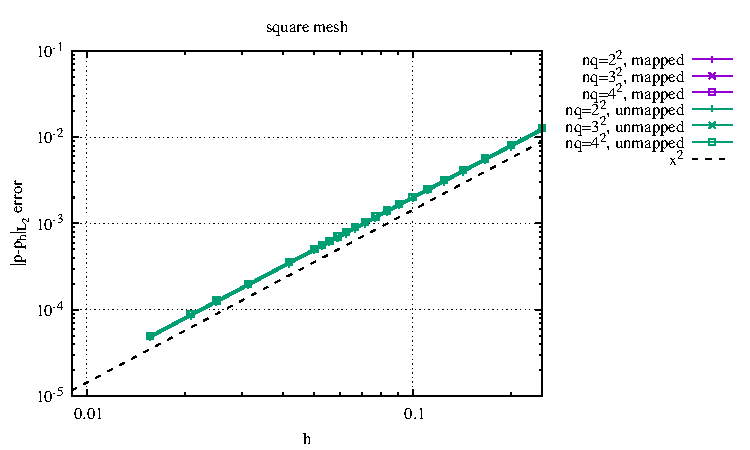
\includegraphics[width=5.7cm]{python_codes/fieldstone_76/results/bench9/reg/errors_P}
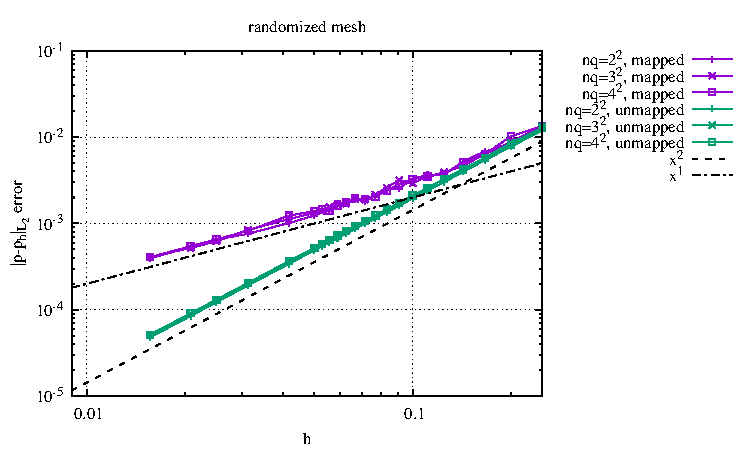
\includegraphics[width=5.7cm]{python_codes/fieldstone_76/results/bench9/rand/errors_P}
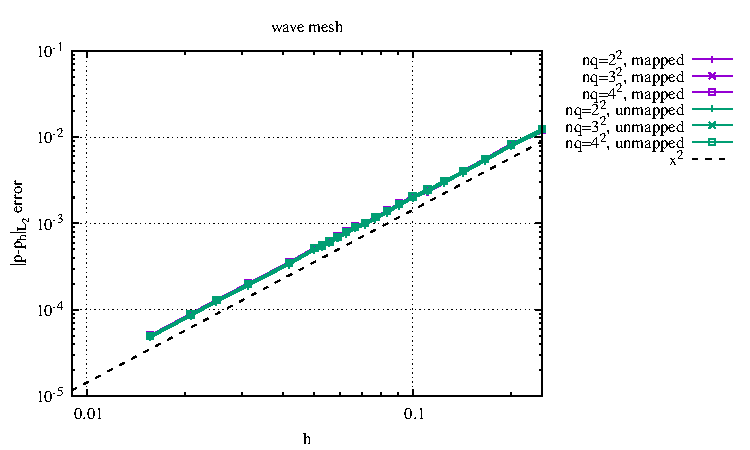
\includegraphics[width=5.7cm]{python_codes/fieldstone_76/results/bench9/wave/errors_P}\\
{\captionfont Left column: Regular square mesh; middle column: Randomized $\xi=0.1$ mesh;
right column: wave mesh.}
\end{center}


\newpage
%.......................................................
\subsection*{Instantaneous sinking block}

It is fully described in Section~\ref{MMM-ss:sinking_block}

\begin{center}
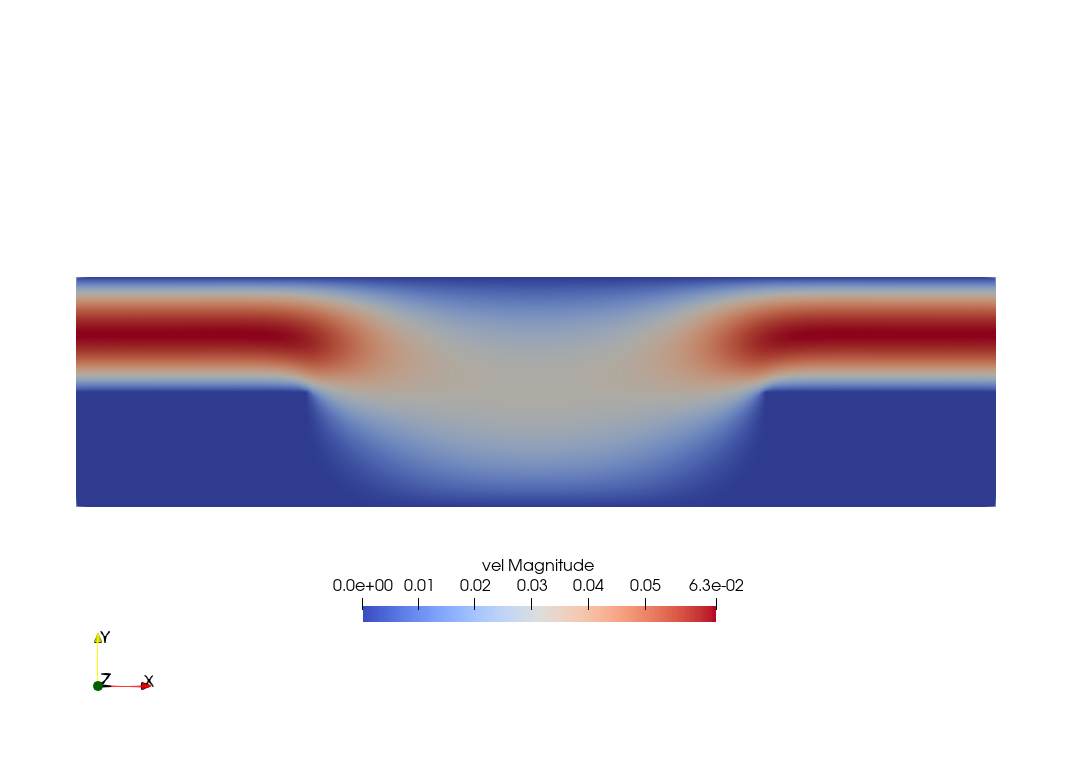
\includegraphics[width=7cm]{python_codes/fieldstone_76/results/block/vel}
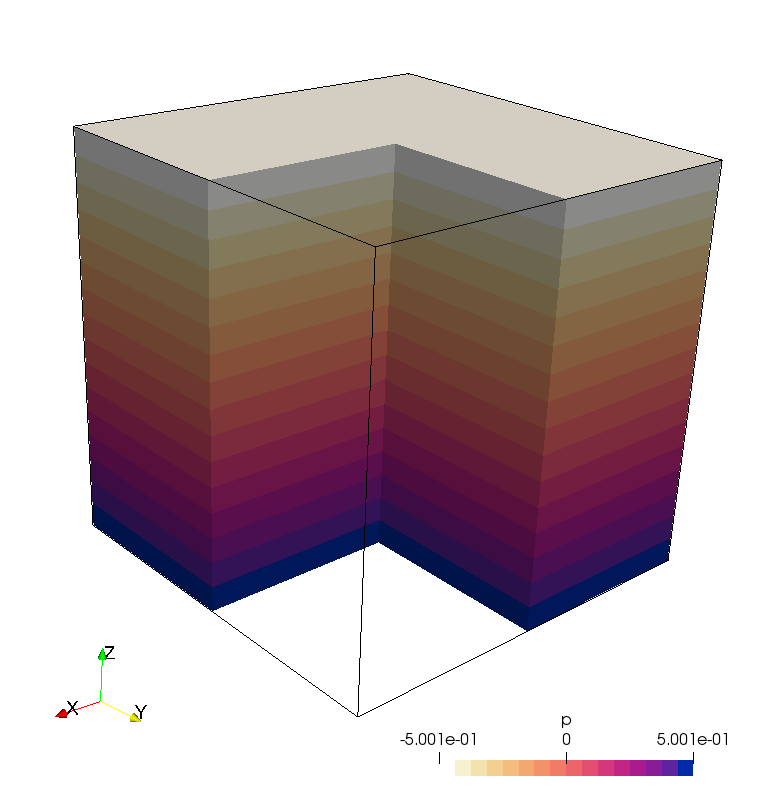
\includegraphics[width=7cm]{python_codes/fieldstone_76/results/block/press}
\end{center}


